% Chapter Template

\chapter{Literature Review} % Main chapter title

\label{Chapter 2} % Change X to a consecutive number; for referencing this chapter elsewhere, use \ref{ChapterX}

Since the introduction of general-purpose mobile operating systems, such as Symbian, Android, Windows 10 and iOS, and especially throughout the last decade, mobile phones have evolved dramatically \cite{Reference1}.
The introduction of feature-rich and complex operating system has not only brought the benefits of a computer, but also the risks of one too \cite{Reference2}.
Since phones have become computerised people have become more trusting of what data they can store on their phone, such as location, bank details, etc \cite{Reference3}.
With private data increasingly being stored on phones, it becomes necessary for mobile security to receive a larger amount of attention.
This literature review explores this issue, as follows:
\begin{itemize}
\item{Section \ref{Ch2 Sec1} explores the interrelationship between complexity and security.}
\item{Section \ref{Ch2 Sec2} documents a wide variety of the security threats facing modern computers, with a particular emphasis on mobile devices.}
\item{Section \ref{Ch2 Sec3} relates the application of isolation and compartmentalisation to improve security.}
\item{Section \ref{Ch2 Sec4} documents the history and status of the MEGA65 project, including the historical Commodore 64 platform on which it is based, as well as the recent work towards introducing compartmentalisation and related security features to the platform.}
\end{itemize}

%----------------------------------------------------------------------------------------
%	SECTION 1
%----------------------------------------------------------------------------------------

\section{Complexity and Security}

\label{Ch2 Sec1}

One of the major issues with the current state of security is that the complexity involved is far beyond what any one person can comprehend.
Intel embodies the complexity issue perfectly when examining the number of employees vs the number of transistors on one of their CPUs.\\

\begin{figure}
  \centering
  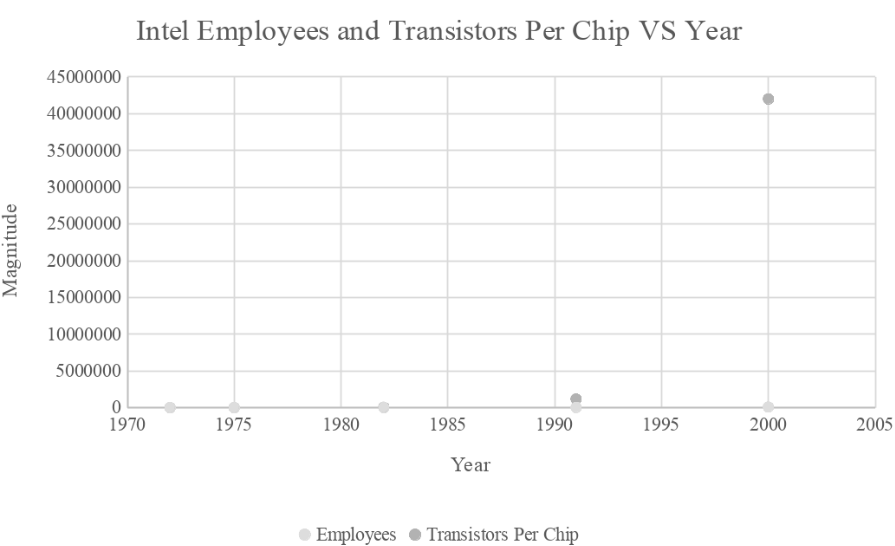
\includegraphics[width=\linewidth]{intelgraph}
  \caption{Graph of Intel's CPU transistor count vs the amount of Intel employees.\\ \cite{Reference28}\cite{Reference29}\cite{Reference30}\cite{Reference31}\cite{Reference32}\cite{Reference33}\cite{Reference34}\cite{Reference35}
}
  \label{fig:intelgraph}
\end{figure}

From 1972 to 2000 Intel’s workforce grew by 86 times, comparing this growth with the transistor growth of 1200 times over the same period, a huge disparity can be seen.
If every employee at Intel was dedicated to testing transistors, in 1972 each employee needed to test 3.5 transistors, compare this to the 487 they need to test now.
This clearly demonstrates the impossibility for, not only one person, but for all of Intel to successfully verify that their CPU is working as intended.
With modern computers unable to be understood by a single person, they are inherently not to be trusted \cite{Reference4}.
Not only are they not to be trusted, but they can never be trusted, because while they are not understood by a single person there is always the possibility of interactions in the CPU that remain undiscovered \cite{Reference5}.\\
As systems become more complex, they too see more issues arise within them.
A key property of this is the amount of failure modes that are present in the system.
Larger, more complex, systems naturally have more security vulnerabilities as they have more interactions, or opportunities for failure \cite{Reference6}.
These larger systems also require more time and effort to test.
More worryingly is that for the end user, this complexity aids malicious attempts \cite{Reference7}.
For the same reasons that testing is difficult, so too is finding indicators of a security breach, or even malicious activity after a breach has been detected \cite{Reference8}.\\
To combat this increase in security flaws there are a few methods that can be used.
One such method is to patch the security flaws with work-arounds.
As these work-arounds were not originally designed as part of the system, there is a possibility that they can make the entire system less secure overall.\\ 
This has been beautifully demonstrated by the recent exploits found in speculative execution processors.
This exploit, named Meltdown, was a massive cause of panic as it allowed privileged information to be read at megabytes a second.
The Windows 7 January 2018 patch for the exploit resulted in permissions for the user being set erroneously.
This allowed the user to read memory that was normally only accessible by the processor \cite{Reference9}.\\
The other method of reducing security flaws is to reduce the complexity of the system.
Less interactions allows more time dedicated to ensuring each one works correctly.
In addition to this, simpler systems allow for users to better understand them, and thus are more easily verified as secure.
This was listed as one of the key aspects of a trusted computer system by the Department of Defence as it is only then that understandable and maintainable protection is achieved \cite{Reference10}.

%----------------------------------------------------------------------------------------
%	SECTION 2
%----------------------------------------------------------------------------------------

\section{Mobile Security Threats}

\label{Ch2 Sec2}

When analysing current mobile (smart) phones there are multiple avenues under which data can be maliciously obtained, or normal service can be disrupted.
These avenues can be categorised under the following labels:
\begin{itemize} 
\item Mobile Hardware
\item Mobile Software
\item Mobile Networks
\item Physical Access
\item Mobile Enterprise 
\end{itemize}

%-----------------------------------
%	SUBSECTION 1
%-----------------------------------

\subsection{Mobile Hardware}

\label{Ch2 Sec2 Sub1}

Mobile hardware refers to the various sensors and physical devices built into the phone.
By accessing the hardware directly on the phone, most software security provided by the operating system is bypassed, allowing malicious users to access data provided by cameras, microphones, etc.
This form of attack is particularly difficult to protect against in some cases due to the advent of users rooting or jail-breaking their phones \cite{Reference11}.
Jail-breaking/rooting is where the user deliberately uses exploits vulnerabilities to gain more control over the phone’s systems.\\
Currently, the best way to defend against mobile hardware exploitation is to ensure that the operating system is up to date and that patches for publicly known exploits are installed.
This does not prevent mobile hardware exploits but rather makes them nontrivial to perform \cite{Reference12}.\\
Even with all the updates and patches installed, there still exists improvements that could be made to further reduce hardware exploits.
As most hardware on a phone does not have an indicator for when it is active, it is difficult to determine its status; implementing this in hardware would allow a user to tell decisively whether hardware was on or off \cite{Reference13}.

%-----------------------------------
%	SUBSECTION 2
%-----------------------------------

\subsection{Mobile Software}

\label{Ch2 Sec2 Sub2}

Mobile software refers mainly to the applications running on the phone, but it  also refers to the background processes that run while the user isn't using their phone.
While these programs give the user more control over their phone, they are also a potential source for coding errors.\\ 
Through these errors such as, files being stored in an unprotected location or files being stored in an insecure format, it is possible to leak sensitive data \cite{Reference14}.
Not only is it possible to read stored data, but through an insecure network or a vulnerable third-party software library, it is possible to read and alter all data being sent to and from the phone.\\ 
To protect against vulnerable software there are limited options available.
Keeping the operating system up to date is the best solution as more security monitoring helps catch exploits \cite{Reference12}.
The process of application analysis involves two different methods, static analysis and dynamic analysis.
In static analysis the source code for an application is evaluated without running it to detect possible exploits.
This method relies on the source code being available, which isn’t always the case, and, if it is computer assisted, can provide false positives \cite{Reference15}.
To a lesser extent, static analysis can be performed on compiled code, but it is limited to program interface, compiler optimisations and software library checking.
Dynamic analysis is like source code static analysis with the exception that it is done with the code running.
This allows behaviour that is not apparent from source code examination to be identified \cite{Reference13}.\\
In addition to coding errors that allow third parties to exploit security vulnerabilities, some applications are developed intentionally for malicious activity.
These less than reputable applications often exploit underlying vulnerabilities in the operating system or trick the user into giving the application privileges that exceed those needed for proper function \cite{Reference16}.\\
Malicious applications can breach phone security in many ways to extort money from the user or gain access to protected data.
Ransomware is the name given to an application that encrypts all the user’s data and demands payment to decrypt it.
This form of extortion poses extreme risk when dealing with cooperate data due to the loss in productivity.
The unauthorised access of user data can be done through many methods such as jail-breaking the phone so that hardware can be exploited, subverting login details, sharing data with other applications (such as Dropbox) and logging private data \cite{Reference13}.\\
Malicious applications are difficult to protect against.
In almost all situations they require some form of active security that is user reliant to effectively protect against them.
In addition to understanding the threats present and keeping all software up to date, users can:\\*
\begin{itemize}
\item Use dynamic analysis in a safe environment
\item Isolate the application from sensitive data
\item Use authentication protocols
\end{itemize}
These methods would allow for adequate protection against malicious applications or applications used for a malicious purpose, but there is still more that can be done.
Better application development practices and regulations would prevent many of the issues with software exploitation.
This is unrealistic though as most applications are so complex there will always be a missed bug.
More transparent applications are the solution to this as it would allow users to not only verify the application but improve upon it \cite{Reference13}.

%-----------------------------------
%	SUBSECTION 3
%-----------------------------------

\subsection{Mobile Networks}

\label{Ch2 Sec2 Sub3}

A mobile network is the interconnection between all phones that allows for phone calls, messages and internet access to the mobile device.
These connections are facilitated by the numerous radios and modem.
The mobile network can be broken down into three major sections, the radio access network, the core network and the external services network.\\
The radio access network facilitates the connection between the mobile device and the service provider for the phone.
This network is used to connect the mobile device to the telephone tower which then leads to the core network.
The core network is responsible for tracking billing, signal routing and connecting the mobile device to the external services network, such as the internet or mobile devices from a different carrier \cite{Reference13}.\\ 
Radio access networks are susceptible to three basic types of exploits, denial of service attacks, eavesdropping and device tracking.
Denial of service attacks is used as a large umbrella term for all the attacks that can block or hinder normal mobile phone operation.
These attacks can be conducted by filling up all available radio access slots on a telephone tower, impersonating a telephone tower to intercept emergency calls or flooding the area with radio waves to obscure legitimate calls \cite{Reference17}.
Eavesdropping, as the name suggests, involves the gaining access to data being transmitted between the telephone tower and mobile device.
This is possible because it is not required that data between the mobile device and the telephone tower be encrypted, in the case that end to end encryption is not used, all the user’s data is free to access by those that can \cite{Reference13}.
For superior data transmission a shorter radio access network is desired, this bring forth a need for mobile device locational services, so the closest radio tower can be used in data transfer.
This can be exploited to track a mobile device and by extension, a user’s location \cite{Reference17}.\\
The core network, once subverted, offers attackers many avenues of attack.
Most mobile networks use some form of management system in order to control the entire network.
This provides the ability to intercept or block phone calls and texts, as well as denying service to users were it subverted \cite{Reference13}.\\
External networks are how a phone connects to the internet among other networks.
This brings all the benefits, but also all the dangers of an internet connection.\\
To defend against data interception and theft, end to end encryption must be used.
This negates any chance of the radio access network and core network leaking data, as the leaked data would still be encrypted.
Denial of service attacks can be mitigated by alternative methods of data transmission.
Though it is highly unlikely that an entire carrier will have it’s services denied, using an alternative method would be able to negate any and all effects of such an attack.
Unfortunately, mobile device tracking cannot be defended against due to it being so intertwined with the mobile network.
Even bouncing a connection across a privately-owned network would not result in much, as it can be traced by a skilled attacker \cite{Reference13}.

%-----------------------------------
%	SUBSECTION 4
%-----------------------------------

\subsection{Physical Access}

\label{Ch2 Sec2 Sub4}

While mobile phones are almost always on person all the time, there are certain situations in which contact must be broken.
These instances occur during certain security checks, like police or airport searches, or during charging and communication sensitive operations.
During these times it would be possible to access data from the phone or perform other malicious activity.\\
One avenue of attack is the combined charging/data port of the phone.
By plugging the phone into a PC, it is possible to abuse vulnerabilities to gain access to data.
This is not limited to PCs however, by modifying a charger with a small PC board it is possible to execute complex attacks on the device whenever the phone is charging.
If done right, this attack could also work in the reverse, infecting a host computer that the phone is connected to \cite{Reference13}.\\
Another avenue is the phone itself, NowSecure released a report in 2016 that stated 43\% of mobile users do not use a pass-code, PIN, or pattern lock on their device \cite{Reference18}.
This, coupled with cached memory and browser cookies could result in banking details, among other things being stolen.\\

The best defence against physical access attacks is to use screen locks and exclusively use personal charging equipment.
These negate the threat of physical access attacks and data port attacks.\\

Despite the ease of ensuring physical security, more needs to be done to encourage users to use this security.
Currently, most phones use authentication methods that don’t fully capitalise on all the mobile sensors available.
While using sensors like fingerprint scanners and facial recognition is emerging in mobile phones, there exists sensors like the capacitive sensor, gyroscope and accelerometer that are still unused in lock screen technology \cite{Reference13}.

%-----------------------------------
%	SUBSECTION 5
%-----------------------------------

\subsection{Mobile Enterprise}

\label{Ch2 Sec2 Sub5}

When mobile devices are integrated into business there comes a need for servers, processes and systems that manage these devices.
This enterprise, such as a company application, can serve as an infection source, should the enterprise itself become infected.
To counteract these flaws mobile device managers for enterprise purposes have been developed.
These managers enforce security policies, remote access, remote wiping, etc. for the device.\\
Because these device managers have a higher level of privilege than the user, exploiting the device manager to gain access to the entire enterprise is a serious threat, as doing so would allow infection of all devices connected to the enterprise.
Once compromised, it is possible for all data within the enterprise to be stolen, manipulated or for all services to be blocked completely.\\
These attacks can be mitigated using comprehensive authentication protocols to prevent impersonation, protected execution environments and network monitoring.
While authentication prevents most forms of attack, it is still subject to authentication information being discovered, which is why the execution environment is used to contain malicious activity and network monitoring is used to look for such activity \cite{Reference13}.

%----------------------------------------------------------------------------------------
%	SECTION 3
%----------------------------------------------------------------------------------------

\section{Security Through Isolation}

\label{Ch2 Sec3}

One approach to securing a computer has been to have sections of it “air gapped”, such that infection in one area cannot affect other areas \cite{Reference19}.\\

One example of an operating system built on this principle is the Qubes OS, which has gone about this through compartmentalisation.
By isolating things, such as untrusted websites, in their own qube it is possible stop any attempt to compromise the whole system as they are contained in that qube.
These qubes are not limited to software, they work with hardware too, meaning that USB controllers and network cards are secured in their own qubes.
This reduces the effectiveness of using hardware as a security exploit \cite{Reference20}.\\

Isolative computing can be emulated by hosting multiple virtual machines on one host machine, thus recreating the Qubes OS concept.
This comes one major disadvantage over using Qubes OS however, once the host OS is subverted all the virtual machines are subverted too \cite{Reference21}.
As Qubes OS uses a hyper-visor to manage all the qubes it is inherently more secure than virtual machine recreation.
This is due to the increased difficulty of subverting the hyper-visor as compared to subverting an operating system.\\

Another method for air gapping a computer is to have it physically isolated from external connections.
By removing the computer from external networks almost all attack vectors are removed too, thus ensuring the computer is safe.
This form of protection is mainly used in critical systems, as by isolating a computer a lot of the functionality of it, such as web browsing, is removed \cite{Reference22}.\\

While air gapping computers appears to make data exfiltration impossible, there are a few ways in which this can happen.
The simplest method is via physical access and a USB or USB device.
The best know device is the USB Rubber Ducky, this device can be used to imitate a keyboard inputs via a script loaded onto the device \cite{Reference23}.
This allows the rubber ducky full control over the host device and can even be used to install malicious software \cite{Reference23}.
Another method of circumventing an air gap is to use high frequency sound from a speaker to transmit and infect air gapped computers \cite{Reference24} “AirHopper” is another method for data exfiltration, instead of using sound, it uses radio waves generated by cables from the computer \cite{Reference25}.
Even when Faraday shielded to prevent these sound and electromagnetic signals from escaping, it is still possible to transmit data from the computer by using the CPU.
The CPU can be used to generate low frequency magnetic waves by altering the load on specific cores.
These magnetic waves more readily penetrate Faraday shielding, allowing the transmission of data from the air gapped computer \cite{Reference26}.

%----------------------------------------------------------------------------------------
%	SECTION 4
%----------------------------------------------------------------------------------------

\section{The MEGA65 Project}

\label{Ch2 Sec4}

The MEGA65 project was born from one Paul Gardner-Stephen in 2014.
The scope of the project was to create an accelerator for the commodore 64.
This changed when the Museum of Electronic Games and Art sponsored the project and connected him with various other experts \cite{Reference27}.
The project was expanded to recreating and archiving the commodore 65, a prototype computer that was never officially released.
In addition to the restoration of this computer, updating the hardware was done wherever possible, so long as they didn’t compromise the identity of the computer \cite{Reference27}.
This was done so an external accelerator was not needed for the project.\\

The MEGA65 computer itself runs on a field programmable gate array (FPGA) dev board.
This option was explored in depth due to a few factors such as, cost, onboard SD card slot, VGA output and the Artix-7 chip.
The cost of boards was a large factor in the decision to use them as they would make the C65 affordable.
The SD card slot on the board also helped this affordability as they are inexpensive and, conveniently, able to easily be interfaced with many computers.
The VGA interface on the board was considered noteworthy as many monitors still have a port for them and there are readily available adaptors for VGA to various other ports \cite{Reference27}.\\

In addition to the MEGA65 project, another project was run along side it, the MEGAphone project.
This project aimed to create a commodore 65 based smart phone with a security focus.
Instead of allowing the technology gap between the MEGAphone and modern phones to be detrimental, it would be one of the key features of the phone.
The vastly simplified way in which the computer worked as well as the age would allow for many advantages over modern systems.\\

The simplicity would allow for the entire device to be verifiable, this is not normally explored by other security development teams.
By being able to verify the phone is working as intended, it becomes almost impossible to compromise.
In addition to this, as the phone is security focused, malicious activity is limited by the phone design itself.
Not only this, but many of the security flaws being found in systems today are just not present in the commodore 64 because it doesn’t have the supporting hardware.

Through the 36 years of activity that the commodore 64 has seen, many bugs have been found and documented in the system.
As such, it is monumentally unlikely that there are new exploits in the system that are unfound, making it excellent to use for security purposes.

